\documentclass[12pt, a4paper]{article}
\usepackage{amsmath}
\usepackage{amsfonts}
\usepackage{fontspec}
\usepackage{graphicx}
\usepackage{float}		%\begin{figure}[H] <- agrega el H
\usepackage{multirow}
\usepackage{multicol}
\usepackage{indentfirst}
\usepackage{caption} %comando \ContinuedFloat
\usepackage{array} %paquete para tabular
\usepackage{subcaption} %subfiguras y continuación de figura
\usepackage{pstricks-add}
\usepackage{bm}
\usepackage{enumitem} %cara utilizar distintos enumerate item
\usepackage{listings} %para poner codigos
\usepackage{esint} %permite usar integrales cerradas


\newcolumntype{P}[1]{>{\centering\arraybackslash}p{#1}} % P{} (mayúscula) en vez de p{} (minúscula)
\newcommand{\vect}[1]{\boldsymbol{#1}} %notación vector \vect{•}
\renewcommand{\contentsname}{Índice}
\renewcommand{\figurename}{Figura}
\renewcommand{\tablename}{Tabla}
\renewcommand\refname{Referencias}

%%% quita los ":" del \caption
\makeatletter
\long\def\@makecaption#1#2{%
\vskip\abovecaptionskip
\sbox\@tempboxa{#1. #2}%
\ifdim \wd\@tempboxa >\hsize
#1. #2\par
\else
\global \@minipagefalse
\hb@xt@\hsize{\hfil\box\@tempboxa\hfil}%
\fi
\vskip\belowcaptionskip}
\makeatother
%%%%%%%%%%%%%%%%%%%%%%%%%


\pagestyle{plain}


%FORMATO PÁGINA
%\hoffset
\voffset=-2cm
\oddsidemargin=0.8cm
%\evensidemargin
%\topmargin 		%entre sup y encab
%\headheight		%tamaño encabezado
%\headsep			%sep encab y text
\textheight=23cm		%altura texto
\textwidth=15cm		%ancho texto
%\marginparsep	%sep notmargen y text
%\marginparwidth	%ancho nota al marg
\footskip=1cm		%pie de pag
\setlength\parindent{0pt}	%sin identacion

\begin{document}

\thispagestyle{empty}

\hspace{-5mm}
\begin{minipage}[c]{7cm}
\centering

\includegraphics[width=4cm]{logoutfsm.jpg} \\
Universidad Técnica Federico Santa María
\end{minipage}
\hfill
\hspace{20mm}
\begin{minipage}[c]{7cm}
\centering

\includegraphics[width=4cm]{logomec1.jpg} \\
Departamento de Ingenieria Mecánica
\end{minipage}

\begin{center}
\vfill
 \Huge{{\bf Proyecto 2 }} \\ 
 \Huge{ {\bf Dinámica de fluidos computacional}} \\ \vspace{1cm}
 \Large{Flujo monofásico newtoniano en una confluencia} \\
 \Large{Parte 1: Discretización de ecuaciones} 
\vfill
\end{center}

\vfill \hfill
\begin{tabular}{l @{ : } l}
Nombre &   Ignacio Apablaza \\
Rol & 201141007-6  \\
Profesores & Romain Gers \\
			& Olivier Skurtys \\
Asignatura & IPM468 \\
\end{tabular}

\newpage
%---------------------------------------------


\tableofcontents


\newpage
%---------------------------------------------

\section{Introducción}

Se estudia el perfil de velocidad de un flujo dentro de una tubería de sección circular. Se emplea el método de volúmenes finitos para la resolución numérica y se contrastan los resultados con los resultados analíticos. \\

En la Sección 2 se estudian los esquemas de discretización flujos convectivos y difusivos, además del esquema de integración temporal a utilizar en la implementación computacional, describiendose de manera general los pasos a seguir en la resolución de la ecuación de Navier-Stokes aplicado a un fluido newtoniano incompresible (Sección 3).\\

Para la integración temporal se emplea un esquema de Euler de orden 2 o esquema de Gear. Esta discretización permite integrar un intervalo de tiempo mediante el método de paso fraccionados o método ADI. En la Sección 4 se nombran algunas consideración al momento de discretizar el dominio físico, para lo cual se utilizan mallas desplazadas (\textit{staggered grid}).  Como se busca obtener un flujo completamente desarrollado se plantea condiciones de borde adecuadas para obtener estas características: Se emplean condición de presión conocida en la entrada y salida del tubo; y condición de periodicidad.\\

Los resultados númericos y teóricos se analizan en la Sección 5. Finalmente se realizan algunas observaciones en la Sección 6.


\newpage
%---------------------------------------------

\section{Ecuación de Navier Stokes discretizado}

Ecuación de Navier-Stokes adimensional para un fluido monofásico, newtoniano e incompresible en coordenadas cartesianas:

\begin{equation}
St \dfrac{\partial v_i^*}{\partial t^*} + v_j^* \dfrac{\partial v_i^*}{\partial x_j^*} = - \dfrac{\partial P^*}{\partial x_i^*} + \dfrac{1}{Re} \Gamma^* \dfrac{\partial^2 v_i^*}{\partial x_j^* \, \partial x_j^*}
\end{equation}

Donde $St$ y $Re$ son los números de Strouhal y Reynolds. El número de Strouhal permite describir el comportamiento oscilatorio de un fluido. Este parametro depende. Si $St \rightarrow 1$ predomina la viscosidad respecto a la oscilación. Suponeniendo obtener un flujo laminar desarrollado se asume $St \approx 1$. Además, como la información de la viscosidad está contenida en el número adimensional $Re$ se simplifica la ecuación haciendo $\Gamma^* = 1$, luego:

\begin{equation}
\dfrac{\partial v_i^*}{\partial t^*} + v_j^* \dfrac{\partial v_i^*}{\partial x_j^*} = - \dfrac{\partial P^*}{\partial x_i^*} + \dfrac{1}{Re} \dfrac{\partial^2 v_i^*}{\partial x_j^* \, \partial x_j^*}
\end{equation}  

Para precindir de la notación ($^*$) se asume que todas las variables a utilizar están adimensionadas


\newpage
%---------------------------------------------

\section{Desarrollo: Discretización de ecuaciones}

Ecuación de conservación/transporte de un escalar pasivo:

\begin{equation} \label{transporte}
\dfrac{\partial \rho \phi}{\partial t} + \nabla \cdot J = \vec{\nabla} P 
\end{equation}

donde $J$ representa la contribución del flujo convectivo y difusivo.

\begin{equation}
J = \rho u \phi - \Gamma \Delta \phi
\end{equation}

Para obtener la formulación en volumenes finitos se aplica el método de residuos ponderados a la ecuación, con soporte compacto y utilizando el método de Galerkin,

\begin{equation}\dfrac{\partial}{\partial t} \iiint_{\Omega_{cv}} \rho \phi d \Omega = - \oiint_{A_{cv}} \vec{F} \cdot \vec{n} d A_n + \iiint_{\Omega_{cv}} S_{\phi} d \Omega
\end{equation}  

Donde

\begin{equation}
\vec{F} = \underbrace{\vec{F}_C}_{\rho \phi \vec{u}} + \underbrace{\vec{F}_D}_{-D \nabla \phi}
\end{equation}

Se recurre al teorema de valor medio representar la integral en función de terminos centrales. Sea $\phi_J$ un valor aproximado que caracteriza al escalar dentro del volumen de control $\Omega_{cv} = \Omega_J$. La ecuación discretizada resulta

\begin{equation}
\dfrac{\partial}{\partial t} \left( \rho \phi_J \Omega_J \right) + \sum \left( F_i \, A_i \right)_J = \left( S_{\phi} \right)_J
\end{equation} 

\subsection{Discretización del flujo convectivo/difusivo en 2D}

Se escoge la discretización propuesta por Patankar \cite{patankar} para dominios en dos dimensiones ($\Delta z = 1$):

\begin{equation} \label{ecuacion_patankar}
\dfrac{\partial \phi}{\partial t} \Delta x \Delta y = a_E \phi_E + a_W \phi_W + a_N \phi_N + a_S \phi_S + a_E \phi_E + a_P \phi_P + b
\end{equation} 

Los coeficientes $a$ están dados por,

\begin{align} \label{coeficientes_patankar}
\begin{split}
a_E &= D_e A(|P_e|) + \mbox{max}(-F_e,0) \\
a_W &= D_w A(|P_w|) + \mbox{max}(F_w,0) \\
a_N &= D_n A(|P_n|) + \mbox{max}(-F_n,0) \\
a_S &= D_s A(|P_s|) + \mbox{max}(F_s,0) \\
a_P &= -a_E -a_W -a_N -a_S \\
b &= S \Delta x \Delta y
\end{split}
\end{align}

\begin{align}
\begin{split}
F_e &= (\rho \, u)_e \, \Delta y \\
F_w &= (\rho \, u)_w \, \Delta y \\
F_n &= (\rho \, v)_n \, \Delta x \\
F_s &= (\rho \, v)_s \, \Delta x
\end{split}
\end{align}

\begin{align}
\begin{split}
D_e &= \dfrac{\Gamma_e}{\Delta x \, \rho \, u_e} \Delta y = \dfrac{1}{Re_e} \Delta y \\
D_w &= \dfrac{\Gamma_w}{\Delta x \, \rho \, u_w} \Delta y = \dfrac{1}{Re_w} \Delta y \\
D_n &= \dfrac{\Gamma_n}{\Delta y \, \rho \, v_n} \Delta x = \dfrac{1}{Re_n} \Delta x \\
D_s &= \dfrac{\Gamma_s}{\Delta y \, \rho \, v_s} \Delta x = \dfrac{1}{Re_s} \Delta x
\end{split}
\end{align}

\begin{align}
\begin{split}
P_e &= \dfrac{F_e}{D_e} \\
P_w &= \dfrac{F_w}{D_w} \\
P_n &= \dfrac{F_n}{D_n} \\
P_s &= \dfrac{F_s}{D_s}
\end{split}
\end{align}

Donde $S$ representa las fuerzas externas independientes de $\phi$. Particularmente estará asociado al gradiente de presión $\vec{\nabla} P$. los términos $F_{nb}$, $D_{nb}$ y $P_{nb}$ están asociados al flujo convectivo, flujo difusivo y el número de Peclet, respectivamente. En la Tabla \ref{tabla_patankar} se exponen distintas fórmulas para calcular la función $A(|P|)$. 

\begin{table} [H]
\centering
\begin{tabular}{|l|l|} \hline
Esquema & Fórmula para $A(|P|)$ \\ \hline \hline
CDS	&	$1-0.5|p|$	\\
UDS	&	$1$	\\
Hybrid	&	$\mbox{max}(0,1-0.5|P|)$	\\
Power law	&	$\mbox{max}(0,(1-0.1|P|)^5)$	\\
Exponential	&	$|P|/\left[ \mbox{exp}(|P|) -1 \right]$ \\ \hline
\end{tabular}
\caption{Funciones de $A(|P|)$ para distintos esquemas de discretización \cite{patankar}. ($P$: número de Peclet)} \label{tabla_patankar}
\end{table}

Este conjunto de ecuaciones discretiza el campo $\phi$ mediante la aplicación de las ecuaciones de conservación de la masa y la ecuación de conservación de la cantidad lineal. Sea $\vec{v} = \{u,v\}^T$ el campo de velocidad en el dominio de control entonces se plantean los sistemas de ecuaciones donde $\phi=u$ y $\phi=v$, donde $u$ y $v$ son escalares asociados a cada malla desplazada (\textit{staggered grid}). Los coeficientes de la ecuación (\ref{ecuacion_patankar}) se calculan de acuerdo a la malla desplaza asociada a la variable $\phi$ a evaluar. Si $\phi = u$, entonces:

\begin{equation}
\dfrac{\partial u}{\partial t} \Delta x \Delta y = a_E^u u_E + a_W^u u_W + a_N^u u_N + a_S^u u_S + a_P^u u_P + b^u
\end{equation} 

Análogo para $\phi = v$

\subsubsection{Término convectivo} \label{convectivo}

Agrupando los términos convectivos de la ecuación \ref{ecuacion_patankar} se obtiene,

\begin{equation}
\begin{split}
H(u) = \underbrace{\mbox{max}(F_w^u,0) u_W \Delta y - (\mbox{max}((F_w^u,0)) + \mbox{max}(-F_e^u,0)) u_P \Delta y + \mbox{max}(-F_e^u,0) u_E \Delta y}_{\partial u^2 / \partial x} + \\ \underbrace{\mbox{max}(F_s^u,0) u_S \Delta x - (\mbox{max}((F_s^u,0)) + \mbox{max}(-F_n^u,0)) u_P \Delta x + \mbox{max}(-F_n^u,0) u_N \Delta x}_{\partial uv / \partial y}
\end{split}
\end{equation}

\begin{equation}
\begin{split}
H(v) =  \underbrace{\mbox{max}(F_w^v,0) v_W \Delta y - (\mbox{max}((F_w^v,0)) + \mbox{max}(-F_e^v,0)) v_P \Delta y + \mbox{max}(-F_e^v,0) v_E \Delta y}_{\partial uv / \partial x} + \\ \underbrace{\mbox{max}(F_s^v,0) v_S \Delta x - (\mbox{max}((F_s^v,0)) + \mbox{max}(-F_n^v,0)) v_P \Delta y + \mbox{max}(-F_n^v,0) v_N \Delta x}_{\partial v^2 / \partial y} 
\end{split}
\end{equation}

Por simplicidad,

\begin{equation}
H(u) = h_W^u u_W + h_E^u u_E + h_S^u u_S + h_N^u u_N + h^u_P u_P
\end{equation}

\begin{equation}
H(v) = h_W^v v_W + h_E^v v_E + h_S^v v_S + h_N^v v_N + h_P^v v_P
\end{equation}

\subsubsection{Término difusivo} \label{difusivo}

Agrupando los términos difusivos de la ecuación \ref{ecuacion_patankar} se obtiene,

\begin{equation}
\begin{split}
G(u) = \dfrac{1}{Re_w^u} A(|P_w^u|) u_W \Delta y + \dfrac{1}{Re_e^u} A(|P_e^u|) u_E \Delta y \\ + \dfrac{1}{Re_s^u} A(|P_s^u|) u_S \Delta x + \dfrac{1}{Re_n^u} A(|P_n^u|) u_N \Delta x \\ - \left[ \left( \dfrac{1}{Re_n^u} A(|P_n^u|) + \dfrac{1}{Re_s^u} A(|P_s^u|) \right) \Delta x \right. \\ + \left. \left( \dfrac{1}{Re_w^u} A(|P_w^u|) + \dfrac{1}{Re_e^u} A(|P_e^u|) \right) \Delta y \right] u_P
\end{split}
\end{equation}

\begin{equation}
\begin{split}
G(v) = \dfrac{1}{Re_w^v} A(|P_w^v|) v_W \Delta y + \dfrac{1}{Re_e^v} A(|P_e^v|) v_E \Delta y \\ + \dfrac{1}{Re_s^v} A(|P_s^v|) v_S \Delta x + \dfrac{1}{Re_n^v} A(|P_n^v|) v_N \Delta x \\ - \left[ \left( \dfrac{1}{Re_n^v} A(|P_n^v|) + \dfrac{1}{Re_s^v} A(|P_s^v|) \right) \Delta x \right. \\ + \left. \left( \dfrac{1}{Re_w^v} A(|P_w^v|) + \dfrac{1}{Re_e^v} A(|P_e^v|) \right) \Delta y \right] v_P
\end{split}
\end{equation}

Por simplicidad,

\begin{equation}
G(u) = g_W^u u_W + g_E^u u_E + g_S^u u_S + g_N^u u_N + g_P^u u_P
\end{equation}

\begin{equation}
G(v) = g_W^v v_W + g_E^v v_E + g_S^v v_S + g_N^v v_N + g_P^v v_P
\end{equation}


\newpage
%---------------------------------------------

\section{Discretización temporal}

Se plantea un esquema BFD2 (\textit{Backward Differentiation Formula 2nd Order}), tambien llamado esquema de Gear. La derivada en (\ref{ecuacion_patankar}) se aproxima mediante,

\begin{equation}
\dfrac{\partial \vec{v}}{\partial t} ^ {n+1} = \dfrac{3 \vec{v}^{n+1} -4\vec{v}^n + \vec{v}^{n-1}}{2 \Delta t} + \Theta(\Delta t^2) 
\end{equation}

El término convectivo en $t_{n+1}$ se obtiene por extrapolación:

\begin{equation}
H(\vec{v}^{n+1}) = 2 H(\vec{v}^n) - H(\vec{v}^{n-1})
\end{equation}

La ecuación a resolver mediante el método de volumenes finitos es:

\begin{equation} \label{ecuación_gobernante}
\dfrac{3 \vec{v}^{n+1} -4\vec{v}^n + \vec{v}^{n-1}}{2 \Delta t} + H(\vec{v}^{n+1}) = -\vec{\nabla} P + G(\vec{v}^{n+1})
\end{equation}

Los pasos a seguir son los siguientes
\begin{enumerate}
\item Predicción del campo de velocidad no solenoidal $\vec{v}^*$
\item Resolución de la ecuación de Poisson sobre la presión
\item Corrección del campo de velocidad
\end{enumerate}

\subsection{Predicción del campo de velocidad no solenoidal $\vec{v}^*$}

\begin{equation}
\dfrac{3 \vec{v}^{*} -4\vec{v}^n + \vec{v}^{n-1}}{2 \Delta t} + H(\vec{v}^{n+1}) = -\vec{\nabla} P + G(\vec{v}^{*})
\end{equation}

Sea $\delta V = \vec{v}^* - \vec{v}^n $ y mediante una manipulación algebráica de la ecuación (\ref{ecuación_gobernante}) se obtiene una ecuación equivalente.

\begin{equation} \label{ecuación_gobernante_modificada}
\left( I - \dfrac{2 \Delta t}{3 \, Re} \Delta \right) \delta V = \dfrac{\vec{v}^n-\vec{v}^{n-1}}{3} - \dfrac{2 \Delta t}{3} \left( H(\vec{v}^{n+1}) + \vec{\nabla} P) \right)
\end{equation} 

Aplicando el método ADI (\textit{Alternating Direction Implicit}) para descomponer al operador de Helmholtz ($I - \frac{2 \Delta t}{3 \, Re} \Delta $)

\begin{equation}
\left( I - \dfrac{2 \Delta t}{3 \, Re} \Delta \right) \approx \left( I - \dfrac{2 \Delta t}{3 \, Re} \dfrac{\partial^2}{\partial y^2} \right) \left( I - \dfrac{2 \Delta t}{3 \, Re} \dfrac{\partial^2}{\partial x^2} \right)
\end{equation}

Luego, resolver (\ref{ecuación_gobernante_modificada}) es equivalente de manera aproximada a resolver

\begin{equation}
\left( I - \dfrac{2 \Delta t}{3 \, Re} \dfrac{\partial^2}{\partial y^2} \right) \underbrace{ \left( I - \dfrac{2 \Delta t}{3 \, Re} \dfrac{\partial^2}{\partial x^2} \right) \delta V }_{\Delta \delta \overline{V}} = \underbrace{ \dfrac{\vec{v}^n-\vec{v}^{n-1}}{3} - \dfrac{2 \Delta t}{3} \left( H(\vec{v}^{n+1}) + \vec{\nabla} P) \right) }_{RHS^n} 
\end{equation}

O bien

\begin{align}
\begin{split}
\left( I - \dfrac{2 \Delta t}{3 \, Re} \dfrac{\partial^2}{\partial x^2} \right) \delta \overline{V} &= RHS^n \\ 
\left( I - \dfrac{2 \Delta t}{3 \, Re} \dfrac{\partial^2}{\partial y^2} \right) \delta V &= \overline{V} \\  
\end{split}
\end{align}

\subsubsection{1er paso en la dirección $x$ ($\delta \overline{V}$)} 

\begin{equation}
\left( I - \dfrac{2 \Delta t}{3 \, Re} \dfrac{\partial^2}{\partial x^2} \right) \delta \overline{V} = \dfrac{\vec{v}^n-\vec{v}^{n-1}}{3} - \dfrac{2 \Delta t}{3} \left( H(\vec{v}^{n+1}) + \vec{\nabla} P) \right) = RHS^n
\end{equation}

Se recurre al método de residuos ponderados,

\begin{equation} \label{primer_paso}
\iiint_{\Omega} \Psi_i \left[ \left( I - \dfrac{2 \Delta t}{3 \, Re}  \dfrac{\partial^2}{\partial x^2} \right) \delta \overline{V}_i - RHS^n \right] \, dV = 0
\end{equation}

Aplicando la formulación para volúmenes finitos y desarrrollando el primer término de la izquierda

\begin{equation}
\iiint_{\Omega_{cv}} \left( I - \dfrac{2 \Delta t}{3 \, Re}  \dfrac{\partial^2}{\partial x^2} \right) \delta \overline{V} \, dV =  \underbrace{\iiint_{\Omega_{cv}} \delta \overline{V} \, dV}_{(**)}  - \underbrace{\dfrac{2 \Delta t}{3 \, Re} \iiint_{\Omega_{cv}}  \dfrac{\partial^2 (\delta \overline{V}) }{\partial x^2} \, dV}_{(***)}
\end{equation}

Resolviendo $(**)$

\begin{equation}
\iiint_{\Omega_{cv}} \delta \overline{V} \, dV =  (\delta \overline{V})_P \, \Delta x \Delta y
\end{equation}

Resolviendo $(***)$

\begin{align*}
\begin{split}
\dfrac{2 \Delta t}{3 \, Re} \iiint_{\Omega_{cv}}  \dfrac{\partial^2 (\delta \overline{V}) }{\partial x^2} \, dV &= \dfrac{2 \Delta t}{3 \, Re} \iint_{\partial \Omega_{cv}} \dfrac{\partial (\delta \overline{V})}{\partial x} \cdot \vec{n} \, dA \\
&= \dfrac{2 \Delta t}{3 \, Re} \left[ -\left(\dfrac{\delta \overline{V}_E - \delta \overline{V}_P}{\Delta x} \right) + \left( \dfrac{\delta \overline{V}_P-\delta \overline{V}_W}{\Delta x} \right) \right] \, \Delta x \Delta y \\
&= \dfrac{2 \Delta t \Delta y}{3 \, Re} \left[ -\delta \overline{V}_E + 2 \delta \overline{V}_P - \delta \overline{V}_W \right]
\end{split}
\end{align*}

Reemplazando $(**)$ y $(***)$ en la (\ref{primer_paso}) se obtiene:

\begin{equation}
(\delta \overline{V})_P \, \Delta x \Delta y - \dfrac{2 \Delta t \Delta y}{3 \, Re} \left[ -\delta \overline{V}_E + 2 \delta \overline{V}_P - \delta \overline{V}_W \right] = \iiint_{\Omega_{cv}} RHS^n \, dV
\end{equation}

El término $RHS^n$ se reemplaza por la ecuación la discretización planteada en la Sección \ref{convectivo} y por el campo de presión definido arbitrariamente a \textit{priori}. La ecuación anterior se traduce en resolver un sistemas de ecuaciones tridiagonal dado por,

\begin{equation}
\begin{split}
\left( \dfrac{2 \Delta t \Delta y}{3 \, Re} \right) \, \delta \overline{V}_E + \left( \Delta x \Delta y - \dfrac{4 \Delta t \Delta y}{3 \, Re} \right) \delta \overline{V}_P + \left( \dfrac{2 \Delta t \Delta x}{3 \, Re} \right) \, \delta \overline{V}_W \\
= \iiint_{\Omega_{cv}} RHS^n \, dV
\end{split}
\end{equation}

\subsubsection{2do paso en la dirección $y$ ($\delta V$)}

Se procede al igual que en el primer paso: 

\begin{equation} \label{segundo_paso}
\iiint_{\Omega} \Psi_i \left[ \left( I - \dfrac{2 \Delta t}{3 \, Re}  \dfrac{\partial^2}{\partial y^2} \right) \delta V_i - \delta \overline{V}_i \right] \, dV = 0
\end{equation}

\begin{equation}
\iiint_{\Omega_{cv}} \left( I - \dfrac{2 \Delta t}{3 \, Re}  \dfrac{\partial^2}{\partial y^2} \right) \delta V \, dV =  \underbrace{\iiint_{\Omega_{cv}} \delta V \, dV}_{('')}  - \underbrace{\dfrac{2 \Delta t}{3 \, Re} \iiint_{\Omega_{cv}}  \dfrac{\partial^2 (\delta \overline{V}) }{\partial y^2} \, dV}_{(''')}
\end{equation}

Resolviendo $('')$
\begin{equation}
\iiint_{\Omega_{cv}} \delta V \, dV =  (\delta V)_P \, \Delta x \Delta y
\end{equation}

Resolviendo $(''')$
\begin{align*}
\begin{split}
\dfrac{2 \Delta t}{3 \, Re} \iiint_{\Omega_{cv}}  \dfrac{\partial^2 (\delta V) }{\partial x^2} \, dV &= \dfrac{2 \Delta t}{3 \, Re} \iint_{\partial \Omega_{cv}} \dfrac{\partial (\delta V)}{\partial y} \cdot \vec{n} \, dA \\
&= \dfrac{2 \Delta t}{3 \, Re} \left[ -\left(\dfrac{\delta V_N - \delta V_P}{\Delta y} \right) + \left( \dfrac{\delta V_P-\delta V_S}{\Delta y} \right) \right] \, \Delta x \Delta y \\
&= \dfrac{2 \Delta t \Delta x}{3 \, Re} \left[ -\delta V_N + 2 \delta V_P - \delta V_S \right]
\end{split}
\end{align*}

Reemplazando $('')$ y $(''')$ en la (\ref{segundo_paso}) se obtiene:

\begin{equation}
(\delta V)_P \, \Delta x \Delta y - \dfrac{2 \Gamma \Delta t \Delta x}{3 \, Re} \left[ -\delta V_N + 2 \delta V_P - \delta V_S \right] = \iiint_{\Omega_{cv}} (\delta \overline{V} ) \, dV
\end{equation}

El término del lado derecho de la ecuación se obtuvo del primer paso de tiempo. Luego, se resuelve el sistema tridiagonal dado por,

\begin{equation}
\begin{split}
\left( \dfrac{2 \Gamma \Delta t \Delta x}{3 \, Re} \right) \, \delta V_N + \left( \Delta x \Delta y - \dfrac{4 \Gamma \Delta t \Delta x}{3 \, Re} \right) \delta V_P + \left( \dfrac{2 \Gamma \Delta t \Delta x}{3 \, Re} \right) \, \delta V_S \\
= \iiint_{\Omega_{cv}} (\delta \overline{V} ) \, dV
\end{split}
\end{equation}

\paragraph{Observación} los pasos anteriores se realizan tanto para $u$ como para $v$ ya que $\vec{v}=\left\{ u,v \right\}^T$ y $\delta V = \vec{v}^* - \vec{v}^n $. Cada paso de tiempo implica resolver 4 sistemas tridiagonales: 2 sistemas para la componente horizontal y 2 sistemas para la componente vertical de la velocidad. Finalmente se obtiene el predictor de la velocidad:

\begin{equation}
\vec{v}^* = \Big| \begin{matrix} u^* = u^n + \delta V_x \\ v^* = v^n + \delta V_y
\end{matrix}
\end{equation}

\subsection{Resolución de la ecuación de Poisson sobre la presión}

\begin{equation}
\Delta \phi = \dfrac{3}{2 \Delta t} \nabla \cdot \vec{v}^*
\end{equation}

\begin{equation}
\phi = \left( P^{n+1} - P^n \right) + \dfrac{1}{Re} \nabla \cdot \vec{v}^* 
\end{equation}

Nuevamente se aplica el método de residuos ponderados con formulación para volúmenes finitos.

\begin{equation}
\iiint_{\Omega} \Psi_i  \left[ \Delta \phi - \dfrac{3}{2 \Delta t} \nabla \cdot v_i^* \right] \, dV = 0
\end{equation}

Luego,

\begin{equation}
\iiint_{\Omega_J} \Delta \phi \, dV = \iiint_{\Omega_J} \dfrac{3}{2 \Delta t} \nabla \cdot v_i^* \, dV
\end{equation}

Recurriendo al teorema de Green-Ostrogradsky se rescribe la ecuación:

\begin{equation}
\iint_{\partial \Omega_J} \vec{\nabla} \phi \vec{n} \, dA = \dfrac{3}{2 \Delta t} \iint_{\partial \Omega_J} \vec{v}^* \cdot \vec{n} \, dA
\end{equation}

\paragraph{Discretización} La función auxiliar $\phi$ se discretiza en la malla desplazada asociada a la presión. Luego, los valores de los flujos de $\phi$ se aproximan en los bordes de cada volumen finito $\Omega_J$, mientras que los valores de las velocidad en $\partial \Omega_J$ son conocidos, sin necesidad de aproximarlos.

\begin{equation}
\begin{split}
\left[ \dfrac{\partial \phi}{\partial x} \Big|_e - \dfrac{\partial \phi}{\partial x} \Big|_w \right] \Delta y + \left[ \dfrac{\partial \phi}{\partial y} \Big|_n - \dfrac{\partial \phi}{\partial y} \Big|_s \right] \Delta x = \\ \dfrac{3}{2 \Delta t} \left( u^*_e - u_w^*  \right) + \dfrac{3}{2 \Delta t} \left( v^*_n - v_s^*  \right)
\end{split}
\end{equation}

Se discretizan las derivadas de $\phi$ implementando un esquemas CDS, obteniendose:

\begin{equation} \label{poisson_discreto}
\begin{split}
\left[ \dfrac{\phi_E-2\phi_P+\phi_W}{\Delta x} \right] \Delta y - \left[ \dfrac{\phi_N-2\phi_P+\phi_S}{\Delta y} \right] \Delta x = \\ \dfrac{3}{2 \Delta t} \left( u_e^* - u_w^* + v_n^* - v_s^* \right)
\end{split}  
\end{equation}

Agrupando los términos $\phi_{nb}$ resulta un sistema de ecuaciones lineales que en forma matricial se representa por una matriz pentadiagonal. Para resolverlo se utiliza el algoritmo TDMA (\textit{Tri-Diagonal MAtrix Algorithm}). Para ellos se define el término $B$ como,

\begin{equation}
B =  \dfrac{3}{2 \Delta t} \left( u_e^* - u_w^* + v_n^* - v_s^* \right)
\end{equation}

Se calcula un predictor (I):

\begin{equation}
\begin{split}
\left( \dfrac{\Delta y}{\Delta x} \right) \phi_E^I - \left( 2 \dfrac{\Delta y}{\Delta x} + 2 \dfrac{\Delta x}{\Delta y} \right) \phi_P^I + \left( \dfrac{\Delta y}{\Delta x} \right) \phi_W^I = \\ \left( \dfrac{\Delta x}{\Delta y} \right) \phi_N + \left( \dfrac{\Delta x}{\Delta y} \right) \phi_S + B
\end{split}
\end{equation}

Se calcula una corrección (II):

\begin{equation}
\begin{split}
\left( \dfrac{\Delta x}{\Delta y} \right) \phi_N^{II} - \left( 2 \dfrac{\Delta y}{\Delta x} + 2 \dfrac{\Delta x}{\Delta y} \right) \phi_P^{II} + \left( \dfrac{\Delta x}{\Delta y} \right) \phi_S^{II} = \\ \left( \dfrac{\Delta y}{\Delta x} \right) \phi_E^I + \left( \dfrac{\Delta y}{\Delta x} \right) \phi_W^I + B
\end{split}
\end{equation}

Un criterio de detención que suele utilizarse en establece lo siguiente: En cada punto de la malla se calcula un residuo $R$ como,

\begin{equation}
R = \sum a_{nb} \phi_{nb} + B - a_P \phi_P 
\end{equation}

La solución converge en la medida que $R$ tiende a cero. Más detalles del algoritmo se explican en \cite{patankar} y \cite{versteeg}. 

\subsection{Correción del campo de velocidad}

Una vez resuelto la ecuación de Poisson se procede a corregir la velocidad predicha en el primer paso:

\begin{equation}
\vec{v}^{n+1} = \vec{v} - \Delta t \nabla \phi
\end{equation}

Se recurre a la misma discretización utilizada en la ecuación (\ref{poisson_discreto}) para el campo auxiliar $\phi$.


\newpage
%---------------------------------------------

\section{Malla Desplazada (Staggered Grid)}

\subsection{Condiciones de contorno}
Se utilizan nodos ficticios para establecer las condiciones de frontera tipo Dirichlet o Neumann. Se utiliza la Figura \ref{fig1} como referencia.

\paragraph{Condiciones de Dirichlet} Utilizando una malla desplaza se observa que para ciertos bordes las condiciones se pueden implementar naturalemente. Sin embargo las condiciones de no deslizamiento en la pared superior no se pueden imponer directamente para $u$ (de la misma manera, en el lado izquierdo del borde no se pueden imponer directamente la condición de $v=0$) Para lograr ello se emplean nodos ficticios que sobresalen los contornos del dominio. Utilizando esquemas CDS se puede imponer que la velocidad $u$ en $\partial \Omega$ sea nulo

\begin{equation}
\dfrac{1}{2} (u + u_f) = 0 \rightarrow u_f = -u
\end{equation}

análogo para la componente vertical

\begin{equation}
\dfrac{1}{2} (v + v_f) = 0 \rightarrow v_f = -v
\end{equation}

El ejemplo se extiende a cualquier valor de velocidad $\vec{v} = \left\{ \overline{u}, \overline{v} \right\}$ en el contorno

\paragraph{Condiciones de Neumann} Se utiliza la misma lógica para imponer las condiciones de flujo en los contornos. Por ejemplo, para la variable $u$ se fija una condiciones de flujo nulo en los contornos y empleando un esquema CDS en el lado izquierdo se tiene:

\begin{equation}
\dfrac{\partial \hat{u}}{\partial x} \Big|_{\Gamma_u} \approx \dfrac{\hat{u}-\hat{u}_f}{\Delta x} = 0  \rightarrow  \hat{u}_f = \hat{u}
\end{equation}

\begin{figure} [H]
\centering
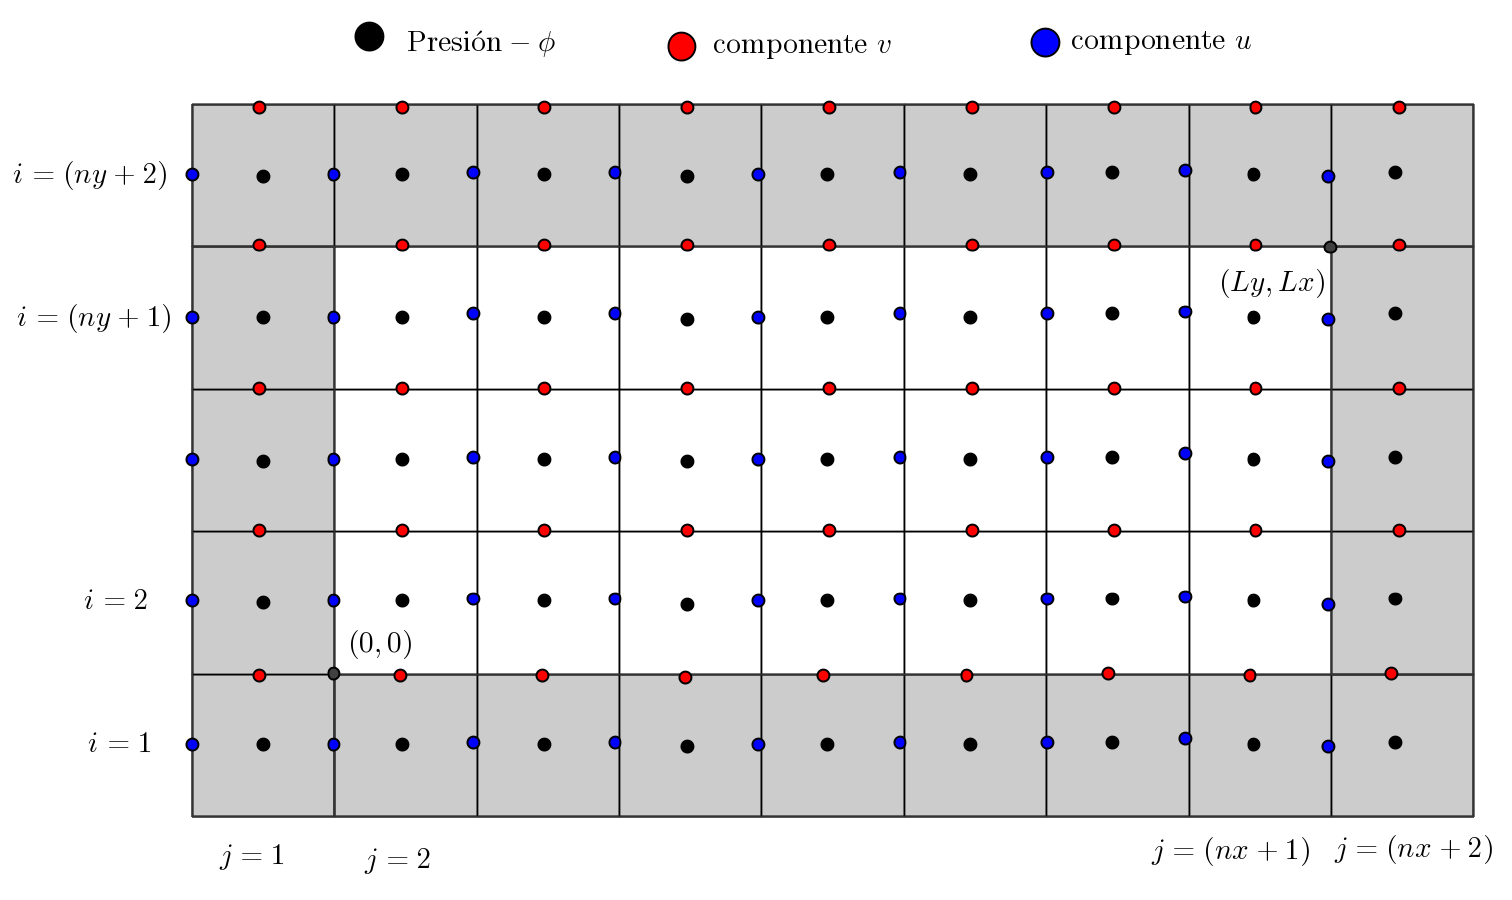
\includegraphics[width=0.8\textwidth]{malla.png}
\caption{Esquema representativo. Círculos azules: $u$ ; Rectángulos rojos: $v$ ; Equis : $P$} \label{fig1}
\end{figure}
\newpage
%---------------------------------------------

\section{Plan de trabajo}

\subsection{Perfil de Poiseuille}

Se busca que en la confluencia exista un flujo de entrada con régimen laminar. Para ello se escoge como volumen de control la entrada de la tubería, como se muestra en la Figura \ref{f2}. La condiciones de contorno son: 
\begin{itemize}
\item Velocidad entrada constante en la entrada
\item Condición de flujo nulo en la salida ($\partial u / \partial x = 0 \rightarrow u = cte$)
\end{itemize}

Utilizando la metodología antes expuesta se busca calcular el perfil de velocidad a la salida del volumen de control. Una vez obtenido el perfil de velocidad se puede trabajar en la confluencia

\begin{figure}[H]
\centering
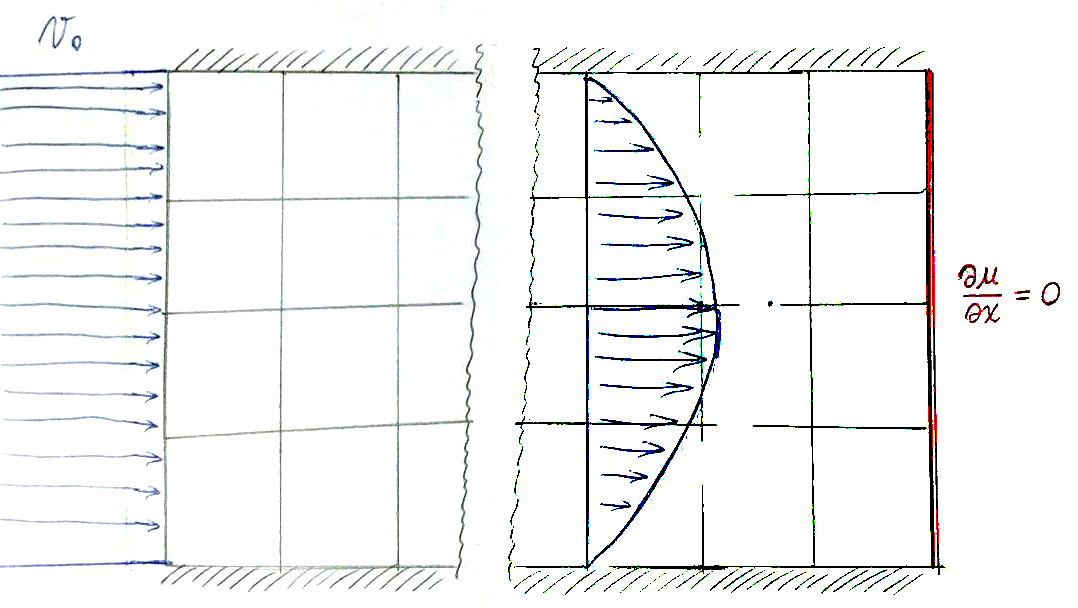
\includegraphics[width=0.8\textwidth]{f2.png}
\caption{ } \label{f2}
\end{figure}

\subsection{Confluencia}

Con el perfil de velocidad previamente calculado a la salida de la tubería, naturalmente se impone el mismo perfil como condición de entrada en la confluencia en ambos extremos, como se ve en la Figura \ref{f3}. De esta manera la resolución del problema es computacionalmente más sencilla y sin perder sustento físico. \\

Se resuelve el campo de velocidad dentro del volumen de control $\Omega$. Conociendo el $\vec{v}$ en cada punto se emplea la ecuación de conservación/transporte de un escalar pasivo (ecuación (\ref{transporte})). Por ejemplo, se puede imponer $C=0$ en $t=0$, y tener un sumidero constante $C=1$ en una o en las dos entradas de la confluencia (ver Figura). Calcular el campo $C(x,y)$ permite visualizar el comportamiento del fluido.

\begin{figure}[H]
\centering
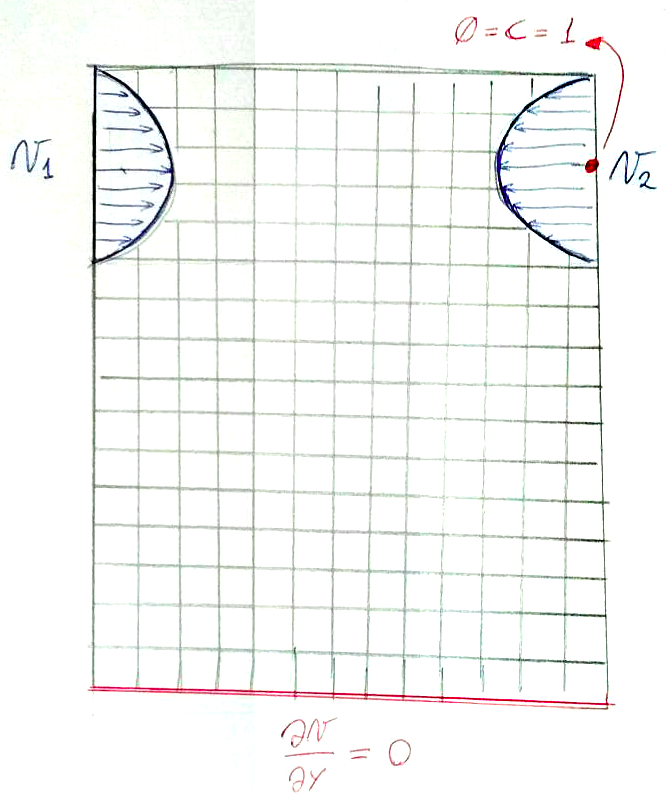
\includegraphics[width=0.8\textwidth]{f3.png}
\caption{ } \label{f3}
\end{figure}
\newpage
%---------------------------------------------

\begin{thebibliography}{3}

\bibitem{patankar} \textsc{Patankar, .S.} , \textit{Numerical Heat Transfer and Fluid Flow, (Series in computational methods in mechanics and thermal sciences)}, Taylor \& Francis, ISBN 0-89116-522-3

\bibitem{versteeg} \textsc{Versteeg, H., Malalasekera, W.,} , \textit{An introduction to Computational Fluid Dynamics}, John Wiley \& Sons Inc., 1995, ISBN 0-582-21884-5

\bibitem{inv} \textsc{Ferziger, J., Peric, M.,} , \textit{Computational Methods for Fluid Dynamics}, Springer, 2002, ISBN 3-540-42074-6

\bibitem{inv} \textsc{Liu, G., R.,} , \textit{Meshfree Methods: Moving Beyond the Finite Element Method}, CRC Press ,2010, ISBN 978-1-4200-8209-8


\end{thebibliography}

\end{document}